\documentclass[a4paper]{article}

\usepackage[french]{babel}
\usepackage[T1]{fontenc}
\usepackage[utf8]{inputenc}
\usepackage{amsmath}
\usepackage{graphicx}
\usepackage{lmodern}
\usepackage[left=3cm, right=3cm, bottom=4cm, top=4cm]{geometry}
\usepackage{array}
\usepackage{pdfpages}
\usepackage{rotating}
\usepackage[gen]{eurosym}
\DeclareUnicodeCharacter{20AC}{\euro{}}
\setcounter{tocdepth}{2}

\usepackage{hyperref}

\title{
\textsc{Jeu SmallWorld\\
\LARGE Manuel d'utilisation}
}

\author
{
	Hyuk-Chan {\sc Kwon}\\
    Florent {\sc Mallard}\\
}

\date{\today}

\begin{document}
	\maketitle
	\begin{center}
		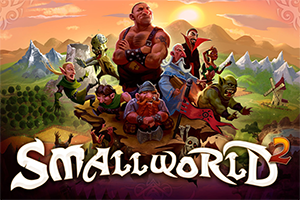
\includegraphics[width=0.8\textwidth]{../../IHM/textures/StartScreen.png}~\\[5cm]
	\end{center}

\newpage
\tableofcontents
\newpage

\section*{Introduction}
Ce jeu est inspiré de SmallWorld. Il s'agit d'un jeu de stratégie à deux joueurs dans lequel chacun dirige un peuple. Les unités des peuples bougent sur les cases de la carte afin de les conquérir, et combattent les unités ennemies. Le but est de contrôler plus de cases que son adversaire.\\

\section{Principes et But du jeu}
	\subsection{Règles du jeu}
		\subsubsection{Peuples}
		Les joueurs ont le choix entre trois peuples : les Orcs, les Elfs et les Nains. Chacun dispose de bonus et malus influant sur la façon de les jouer.

\paragraph{Elfs} Les Elfs ont un coût de déplacement réduit de moitié sur une case Forêt, tandis que le déplacement sur une case Déserte est deux fois plus coûteux. Lors d'un combat dont l'issue conduit à la mort de l'unité, celle-ci a 50\% de chance de s'échapper avec 1 point de vie.
\paragraph{Orcs} Les Orcs ont un coût de déplacement de 50\% sur une case Plaine. Ils ne gagnent aucun point sur une case Forêt, mais ont un bonus propre à l'unité lorsque celle-ci en tue une autre.
\paragraph{Nains} Les Nains ont un coût de déplacement divisé par deux sur une case Plaine. Ils n'acquièrent aucun point sur les cases de ce type. Ils peuvent se déplacer d'une case Montagne à une autre à condition que celle-ci ne soit pas occupée par une unité adverse.

		\subsubsection{Cartes}
		Le joueur, à la création de la partie, a le choix entre trois cartes :
		\begin{itemize}
			\item Small : 2 joueurs, 5 cases x 5 cases, 5 tours, 4 unités par peuple.
			\item Medium : 2 joueurs, 10 cases x 10 cases, 20 tours, 6 unités par peuple.
			\item Large : 2 joueurs, 15 cases x 15 cases, 30 tours, 8 unités par peuple.
		\end{itemize}

		\subsubsection{Déroulement d'une partie}
		Au début du jeu, chaque joueur choisit son peuple. Chaque peuple débute la partie avec toutes ses unités sur la même case de la carte, choisie de manière à ce que les joueurs ne soient pas trop proches. L’ordre de jeu est déterminé aléatoirement en début de partie. Les joueurs jouent chacun leur tour sur le même ordinateur.

	\subsection{Tours de jeu}
	Lorsqu’un joueur peut jouer (c.-à-d. une fois par tour), il peut déplacer toutes ses unités suivant leur nombre de points de déplacement (à part dans le cas d'un bonus lié au peuple, un déplacement sur une case coûte un point de déplacement). Une unité combattante peut engager un combat s’il lui reste au moins un point de mouvement. Une fois le tour terminé, c’est au joueur suivant de commencer son tour. La partie se termine lorsque le nombre de tours prédéfini en début de partie a été effectué, ou lorsqu’il ne reste qu’un seul joueur sur le plateau.

\section{Guide d'utilisation}
	\subsection{Lancement du jeu}
	Pour lancer le jeu, allez dans SmallWorld/IHM et lancez \og IHM.exe \fg{}. Une fenêtre s'ouvre alors dans laquelle vous pouvez choisir de lancer une nouvelle partie ou bien en charger une existante, comme montré sur la Figure \ref{fig:lancement}.
	\begin{figure}[h!]
		\centering
		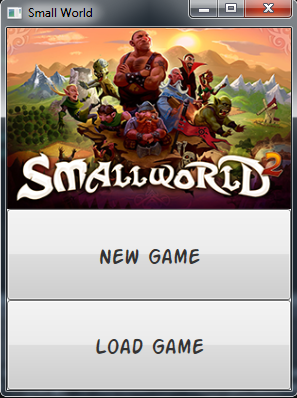
\includegraphics[width=0.4\textwidth]{../../IHM/lancement.png}
		\caption{Fenêtre de lancement du jeu}
		\label{fig:lancement}		
	\end{figure}

		\subsubsection{Nouvelle partie}
		En cliquant sur le bouton \og New Game\fg{} vous pourrez choisir le nom des joueurs ainsi que les peuples que vous désirez jouer. Cette interface est représentée à la Figure \ref{fig:settings}.
		Vous pourrez ensuite lancer la partie en cliquant sur \og Start\fg{}.
		\begin{figure}[h!]
			\centering
			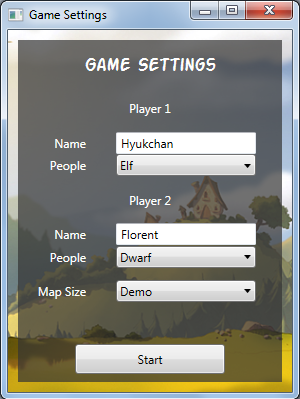
\includegraphics[width=0.4\textwidth]{../../IHM/settings.png}
			\caption{Ecran de configuration de la partie.}
			\label{fig:settings}
		\end{figure}

		\newpage\subsubsection{Chargement d'une partie}
		En cliquant sur le bouton \og Load Game\fg{} vous pourrez choisir la partie à charger. Cet écran est représenté à la Figure \ref{fig:loading}. Les sauvegardes sont effectuées dans le dossier SmallWorld/Small World/IHM/bin/Debug.
		\begin{figure}[h!]
			\centering
			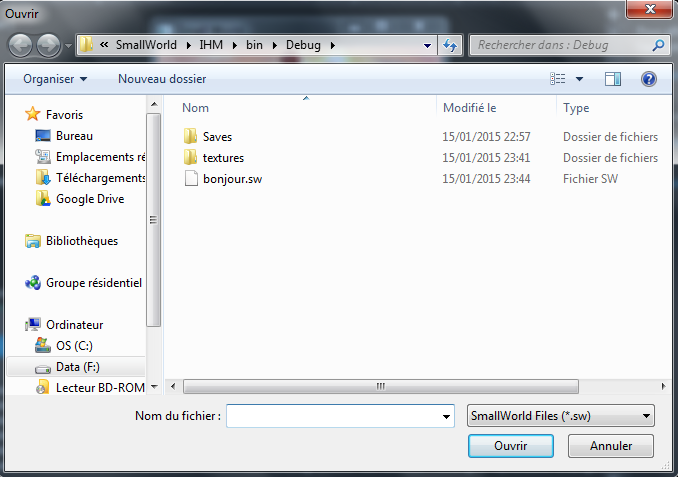
\includegraphics[width=0.8\textwidth]{../../IHM/loading.png}
			\caption{Chargement d'une partie.}
			\label{fig:loading}
		\end{figure}


	\subsection{Interface du jeu}
	Une fois la partie lancée, l'écran suivant s'affiche :
		\begin{figure}[h!]
			\centering
			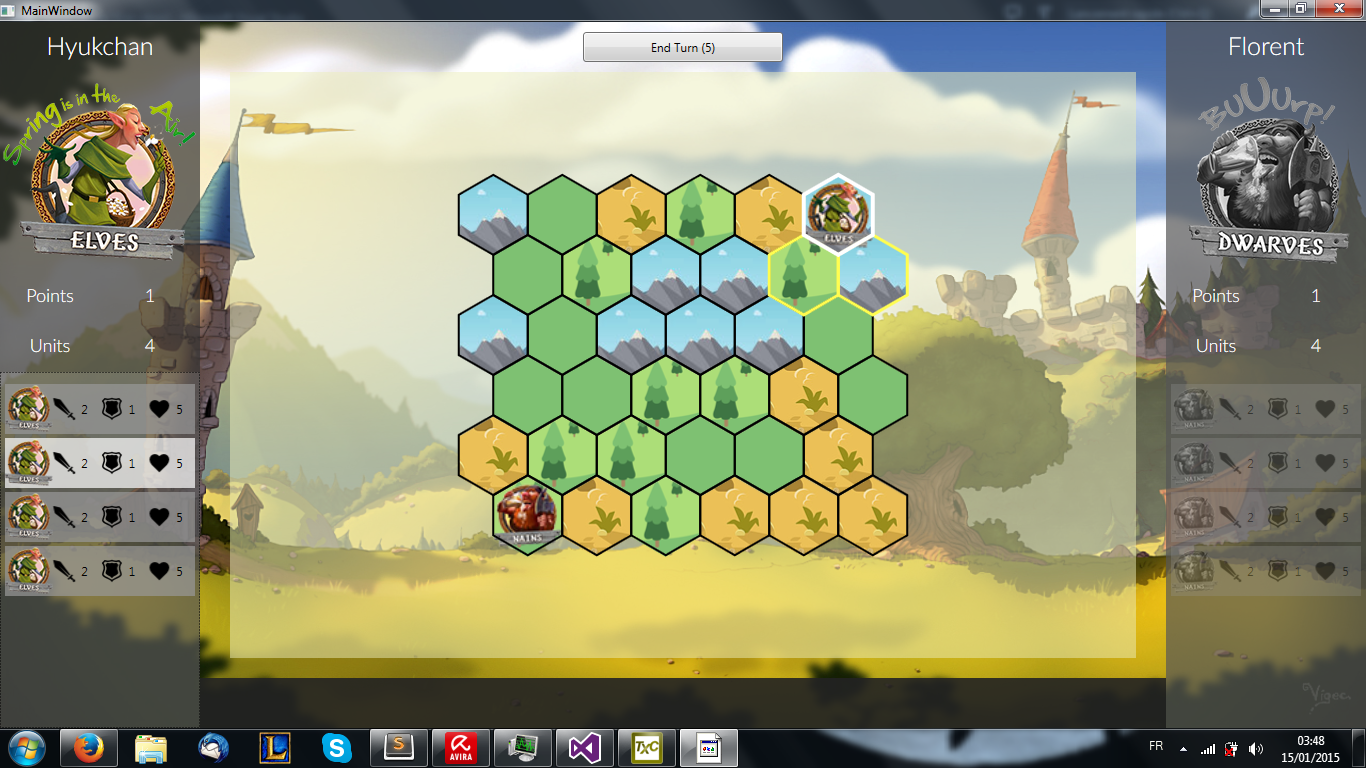
\includegraphics[width=\textwidth]{../../IHM/partie_lancee.png}
			\caption{Partie lancée.}
			\label{fig:debut_partie}
		\end{figure}

		\subsubsection{Panneaux latéraux}
		Les deux joueurs, leur peuple et leurs unités sont représentés de chaque côté de la fenêtre. Les joueurs ont également connaissance de leur nombre de points et d'unités restantes.
		Le joueur dont le tour est en cours est coloré, et ses unités disponibles également.

		\subsubsection{Carte}
		Lorsqu'une case est sélectionnée, elle est entourée de blanc. Si la case contient une de vos unités, elle est automatiquement sélectionnée et ses déplacements disponibles sont colorés en jaune. Si elle en contient plusieurs, une seule est sélectionnée, ses déplacements affichés, et les autres unités sur la case sont en légère surbrillance.

		\subsubsection{Panneau supérieur}
		Au-dessus de la carte, le nombre de tours restant avant la fin de la partie est rappelé. C'est également dans ce panneau que les joueurs pourront terminer leur tour en appuyant sur le bouton \og End Turn\fg{}.

		\subsubsection{Panneau inférieur}
		Ce panneau contient le résumé des dernières actions marquantes. Il affiche entre autres les erreurs effectuées par le joueur courant, les pertes de points de vie lors d'un combat et les décès d'unités.
		\begin{figure}[h!]
			\centering
			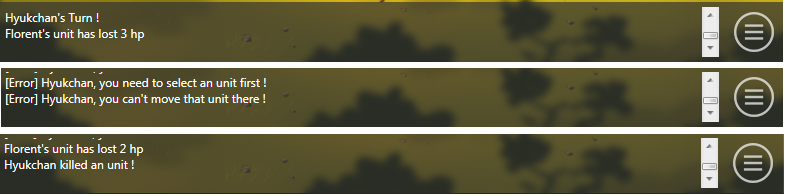
\includegraphics[width=0.9\textwidth]{../../IHM/info.png}
			\caption{Informations données par le jeu.}
			\label{fig:infos}
		\end{figure}

		Le menu est accessible depuis ce panneau (bouton rond situé à droite de la barre de défilement). Celui-ci ouvre un menu permettant de quitter, sauvegarder la partie ou reprendre le jeu, comme illustré à la Figure \ref{fig:menu}.
		\begin{figure}[h!]
			\centering
			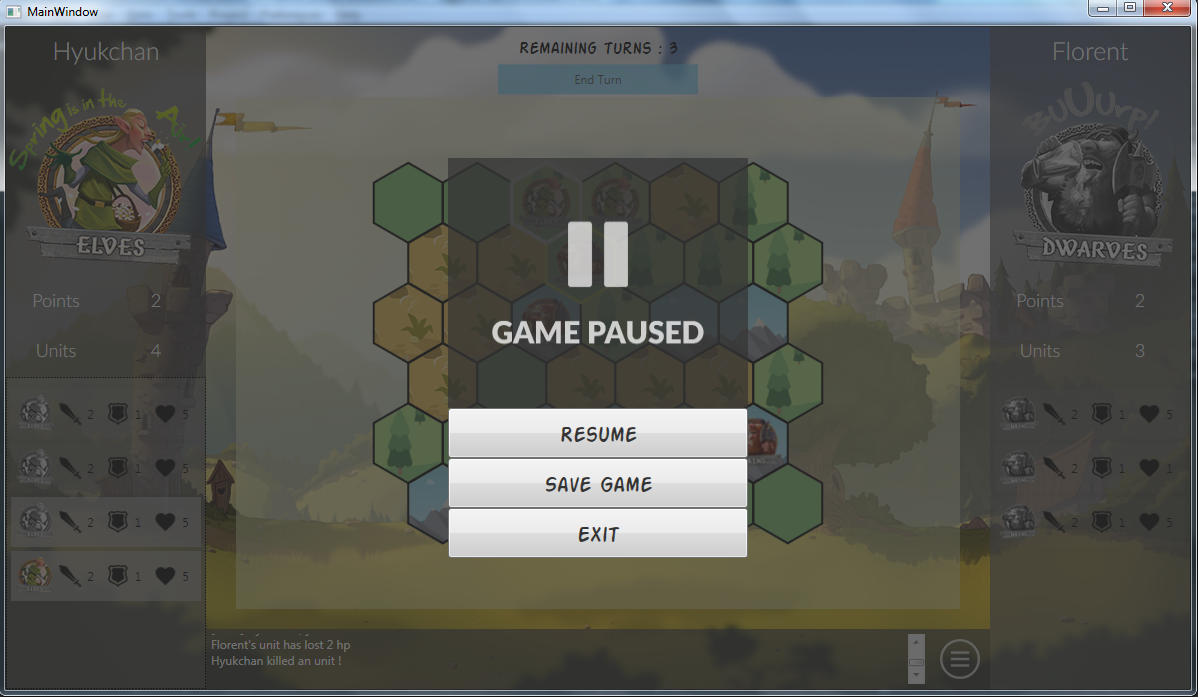
\includegraphics[width=0.9\textwidth]{../../IHM/menu.png}
			\caption{Menu de pause.}
			\label{fig:menu}
		\end{figure}

		\subsubsection{Menu et sauvegarde}
		Le bouton \og Exit \fg{} renvoie au menu principal permettant de créer ou charger une partie. Le bouton \og Save \fg{} permet de choisir le nom de sa sauvegarde. (voir à la Figure \ref{fig:save})
		\begin{figure}[h!]
			\centering
			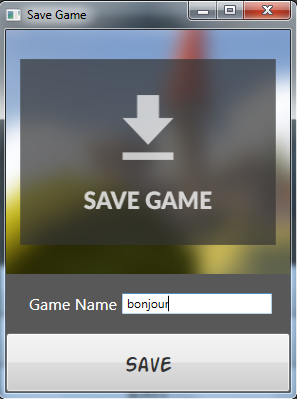
\includegraphics[width=0.45\textwidth]{../../IHM/save.png}
			\caption{Menu de sauvegarde.}
			\label{fig:save}
		\end{figure}

		Une fenêtre s'ouvre pour indiquer que la sauvegarde a bien été effectuée.
		\begin{figure}[h!]
			\centering
			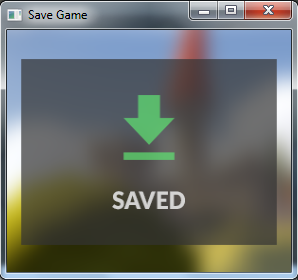
\includegraphics[width=0.45\textwidth]{../../IHM/saveOk.png}
			\caption{Sauvegarde réussie.}
			\label{fig:saveOk}
		\end{figure}

		\newpage\subsubsection{Fin de la partie}
		La partie se termine quand l'un des deux joueurs n'a plus d'unité ou si le nombre de tours impartis a été joué. Dans ce cas, une fenêtre indiquant l'éventuel vainqueur s'affiche, et propose de quitter le jeu ou de recommencer une partie en retournant au menu d'accueil. Ces choix sont décrits par la Figure \ref{fig:fin}.
		\begin{figure}[h!]
			\centering
			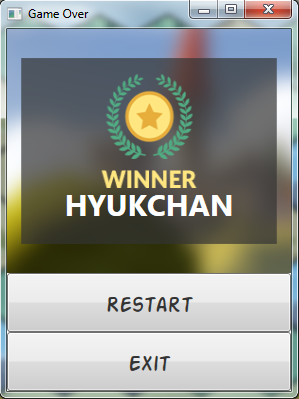
\includegraphics[width=0.45\textwidth]{../../IHM/fin.png}
			\caption{Hyuk-Chan est le vainqueur.}
			\label{fig:fin}
		\end{figure}

	\newpage\subsection{Commandes spéciales}
		\subsubsection{Déplacements}
		Pour vous déplacer, il vous faut sélectionner une de vos unités. Vous pouvez pour cela effectuer un clic gauche sur la case où se situe l'unité que vous voulez déplacer, ou effectuer un clic gauche directement sur l'unité désirée dans le panneau latéral.

		Si le déplacement n'est pas possible, cela sera indiqué dans le panneau inférieur.

		\subsubsection{Combats}
		Les combats sont gérés par le jeu. Ils interviennent automatiquement lorsqu'une unité peut se déplacer sur une case contenant des unités adverses, et que ce déplacement est demandé. Les nains ne peuvent cependant pas attaquer une unité à distance, et ce même si les opposants sont sur une case \og Montagne \fg{}.

\end{document}